\documentclass[11pt,fleqn]{book} % Default font size and left-justified equations
\usepackage{amssymb}
\usepackage{indentfirst}
\usepackage[top=3cm,bottom=3cm,left=3.2cm,right=3.2cm,headsep=10pt,letterpaper]{geometry} % Page margins
\usepackage{xcolor,lipsum} % Required for specifying colors by name
\definecolor{ocre}{RGB}{51,102,0} 
\definecolor{lightgray}{RGB}{229,229,229} 
% Font Settings
\usepackage{avant} % Use the Avantgarde font for headings
%\usepackage{times} % Use the Times font for headings
\usepackage{mathptmx} % Use the Adobe Times Roman as the default text font together with math symbols from the Sym­bol, Chancery and Com­puter Modern fonts

\usepackage{microtype} % Slightly tweak font spacing for aesthetics
\usepackage[utf8]{inputenc} % Required for including letters with accents
\usepackage[T1]{fontenc} % Use 8-bit encoding that has 256 glyphs


% MATHS PACKAGE
\usepackage{amsmath,tikz}
\usetikzlibrary{matrix}
\newcommand*{\horzbar}{\rule[0.05ex]{2.5ex}{0.5pt}}
\usepackage{calc}

% VERBATIM PACKAGE
\usepackage{verbatim}

% Bibliography
\usepackage[style=alphabetic,sorting=nyt,sortcites=true,autopunct=true,babel=hyphen,hyperref=true,abbreviate=false,backref=true,backend=biber]{biblatex}
\addbibresource{bibliography.bib} % BibTeX bibliography file
\defbibheading{bibempty}{}

%----------------------------------------------------------------------------------------
%	VARIOUS REQUIRED PACKAGES
%----------------------------------------------------------------------------------------

\usepackage{titlesec} % Allows customization of titles

\usepackage{graphicx} % Required for including pictures
\graphicspath{{Pictures/}} % Specifies the directory where pictures are stored

\usepackage{lipsum} % Inserts dummy text

\usepackage{tikz} % Required for drawing custom shapes

\usepackage[english]{babel} % English language/hyphenation

\usepackage{enumitem} % Customize lists
\setlist{nolistsep} % Reduce spacing between bullet points and numbered lists

\usepackage{booktabs} % Required for nicer horizontal rules in tables

\usepackage{eso-pic} % Required for specifying an image background in the title page

%----------------------------------------------------------------------------------------
%	MAIN TABLE OF CONTENTS
%----------------------------------------------------------------------------------------

\usepackage{titletoc} % Required for manipulating the table of contents

\contentsmargin{0cm} % Removes the default margin
% Chapter text styling
\titlecontents{chapter}[1.25cm] % Indentation
{\addvspace{15pt}\large\sffamily\bfseries} % Spacing and font options for chapters
{\color{ocre!60}\contentslabel[\Large\thecontentslabel]{1.25cm}\color{ocre}} % Chapter number
{}  
{\color{ocre!60}\normalsize\sffamily\bfseries\;\titlerule*[.5pc]{.}\;\thecontentspage} % Page number
% Section text styling
\titlecontents{section}[1.25cm] % Indentation
{\addvspace{5pt}\sffamily\bfseries} % Spacing and font options for sections
{\contentslabel[\thecontentslabel]{1.25cm}} % Section number
{}
{\sffamily\hfill\color{black}\thecontentspage} % Page number
[]
% Subsection text styling
\titlecontents{subsection}[1.25cm] % Indentation
{\addvspace{1pt}\sffamily\small} % Spacing and font options for subsections
{\contentslabel[\thecontentslabel]{1.25cm}} % Subsection number
{}
{\sffamily\;\titlerule*[.5pc]{.}\;\thecontentspage} % Page number
[] 

%----------------------------------------------------------------------------------------
%	MINI TABLE OF CONTENTS IN CHAPTER HEADS
%----------------------------------------------------------------------------------------

% Section text styling
\titlecontents{lsection}[0em] % Indendating
{\footnotesize\sffamily} % Font settings
{}
{}
{}

% Subsection text styling
\titlecontents{lsubsection}[.5em] % Indentation
{\normalfont\footnotesize\sffamily} % Font settings
{}
{}
{}
 
%----------------------------------------------------------------------------------------
%	PAGE HEADERS
%----------------------------------------------------------------------------------------

\usepackage{fancyhdr} % Required for header and footer configuration

\pagestyle{fancy}
\renewcommand{\chaptermark}[1]{\markboth{\sffamily\normalsize\bfseries\chaptername\ \thechapter.\ #1}{}} % Chapter text font settings
\renewcommand{\sectionmark}[1]{\markright{\sffamily\normalsize\thesection\hspace{5pt}#1}{}} % Section text font settings
\fancyhf{} \fancyhead[LE,RO]{\sffamily\normalsize\thepage} % Font setting for the page number in the header
\fancyhead[LO]{\rightmark} % Print the nearest section name on the left side of odd pages
\fancyhead[RE]{\leftmark} % Print the current chapter name on the right side of even pages
\renewcommand{\headrulewidth}{0.5pt} % Width of the rule under the header
\addtolength{\headheight}{2.5pt} % Increase the spacing around the header slightly
\renewcommand{\footrulewidth}{0pt} % Removes the rule in the footer
\fancypagestyle{plain}{\fancyhead{}\renewcommand{\headrulewidth}{0pt}} % Style for when a plain pagestyle is specified

% Removes the header from odd empty pages at the end of chapters
\makeatletter
\renewcommand{\cleardoublepage}{
\clearpage\ifodd\c@page\else
\hbox{}
\vspace*{\fill}
\thispagestyle{empty}
\newpage
\fi}

%----------------------------------------------------------------------------------------
%	THEOREM STYLES
%----------------------------------------------------------------------------------------

\usepackage{amsmath,amsfonts,amssymb,amsthm} % For math equations, theorems, symbols, etc

\newcommand{\intoo}[2]{\mathopen{]}#1\,;#2\mathclose{[}}
\newcommand{\ud}{\mathop{\mathrm{{}d}}\mathopen{}}
\newcommand{\intff}[2]{\mathopen{[}#1\,;#2\mathclose{]}}
\newtheorem{notation}{Notation}[chapter]

%%%%%%%%%%%%%%%%%%%%%%%%%%%%%%%%%%%%%%%%%%%%%%%%%%%%%%%%%%%%%%%%%%%%%%%%%%%
%%%%%%%%%%%%%%%%%%%% dedicated to boxed/framed environements %%%%%%%%%%%%%%
%%%%%%%%%%%%%%%%%%%%%%%%%%%%%%%%%%%%%%%%%%%%%%%%%%%%%%%%%%%%%%%%%%%%%%%%%%%
\newtheoremstyle{ocrenumbox}% % Theorem style name
{0pt}% Space above
{0pt}% Space below
{\normalfont}% % Body font
{}% Indent amount
{\small\bf\sffamily\color{ocre}}% % Theorem head font
{\;}% Punctuation after theorem head
{0.25em}% Space after theorem head
{\small\sffamily\color{ocre}\thmname{#1}\nobreakspace\thmnumber{\@ifnotempty{#1}{}\@upn{#2}}% Theorem text (e.g. Theorem 2.1)
\thmnote{\nobreakspace\the\thm@notefont\sffamily\bfseries\color{black}---\nobreakspace#3.}} % Optional theorem note
\renewcommand{\qedsymbol}{$\blacksquare$}% Optional qed square

\newtheoremstyle{blacknumex}% Theorem style name
{5pt}% Space above
{5pt}% Space below
{\normalfont}% Body font
{} % Indent amount
{\small\bf\sffamily}% Theorem head font
{\;}% Punctuation after theorem head
{0.25em}% Space after theorem head
{\small\sffamily{\tiny\ensuremath{\blacksquare}}\nobreakspace\thmname{#1}\nobreakspace\thmnumber{\@ifnotempty{#1}{}\@upn{#2}}% Theorem text (e.g. Theorem 2.1)
\thmnote{\nobreakspace\the\thm@notefont\sffamily\bfseries---\nobreakspace#3.}}% Optional theorem note

\newtheoremstyle{blacknumbox} % Theorem style name
{0pt}% Space above
{0pt}% Space below
{\normalfont}% Body font
{}% Indent amount
{\small\bf\sffamily}% Theorem head font
{\;}% Punctuation after theorem head
{0.25em}% Space after theorem head
{\small\sffamily\thmname{#1}\nobreakspace\thmnumber{\@ifnotempty{#1}{}\@upn{#2}}% Theorem text (e.g. Theorem 2.1)
\thmnote{\nobreakspace\the\thm@notefont\sffamily\bfseries---\nobreakspace#3.}}% Optional theorem note

%%%%%%%%%%%%%%%%%%%%%%%%%%%%%%%%%%%%%%%%%%%%%%%%%%%%%%%%%%%%%%%%%%%%%%%%%%%
%%%%%%%%%%%%% dedicated to non-boxed/non-framed environements %%%%%%%%%%%%%
%%%%%%%%%%%%%%%%%%%%%%%%%%%%%%%%%%%%%%%%%%%%%%%%%%%%%%%%%%%%%%%%%%%%%%%%%%%
\newtheoremstyle{ocrenum}% % Theorem style name
{5pt}% Space above
{5pt}% Space below
{\normalfont}% % Body font
{}% Indent amount
{\small\bf\sffamily\color{ocre}}% % Theorem head font
{\;}% Punctuation after theorem head
{0.25em}% Space after theorem head
{\small\sffamily\color{ocre}\thmname{#1}\nobreakspace\thmnumber{\@ifnotempty{#1}{}\@upn{#2}}% Theorem text (e.g. Theorem 2.1)
\thmnote{\nobreakspace\the\thm@notefont\sffamily\bfseries\color{black}---\nobreakspace#3.}} % Optional theorem note
\renewcommand{\qedsymbol}{$\blacksquare$}% Optional qed square
\makeatother

% Defines the theorem text style for each type of theorem to one of the three styles above
\newcounter{dummy} 
\numberwithin{dummy}{section}
\theoremstyle{ocrenumbox}
\newtheorem{theoremeT}[dummy]{Theorem}
\newtheorem{problem}{Problem}[chapter]
\newtheorem{exerciseT}{Exercise}[chapter]
\theoremstyle{blacknumex}
\newtheorem{exampleT}{Example}[chapter]
\theoremstyle{blacknumbox}
\newtheorem{vocabulary}{Vocabulary}[chapter]
\newtheorem{definitionT}{Definition}[section]
\newtheorem{corollaryT}[dummy]{Corollary}
\theoremstyle{ocrenum}
\newtheorem{proposition}[dummy]{Proposition}

%----------------------------------------------------------------------------------------
%	DEFINITION OF COLORED BOXES
%----------------------------------------------------------------------------------------

\RequirePackage[framemethod=default]{mdframed} % Required for creating the theorem, definition, exercise and corollary boxes

% Theorem box
\newmdenv[skipabove=7pt,
skipbelow=7pt,
backgroundcolor=black!5,
linecolor=ocre,
innerleftmargin=5pt,
innerrightmargin=5pt,
innertopmargin=5pt,
leftmargin=0cm,
rightmargin=0cm,
innerbottommargin=5pt]{tBox}

% Exercise box	  
\newmdenv[skipabove=7pt,
skipbelow=7pt,
rightline=false,
leftline=true,
topline=false,
bottomline=false,
backgroundcolor=ocre!10,
linecolor=ocre,
innerleftmargin=5pt,
innerrightmargin=5pt,
innertopmargin=5pt,
innerbottommargin=5pt,
leftmargin=0cm,
rightmargin=0cm,
linewidth=4pt]{eBox}	

% Definition box
\newmdenv[skipabove=7pt,
skipbelow=7pt,
rightline=false,
leftline=true,
topline=false,
bottomline=false,
linecolor=ocre,
innerleftmargin=5pt,
innerrightmargin=5pt,
innertopmargin=0pt,
leftmargin=0cm,
rightmargin=0cm,
linewidth=4pt,
innerbottommargin=0pt]{dBox}	

% Corollary box
\newmdenv[skipabove=7pt,
skipbelow=7pt,
rightline=false,
leftline=true,
topline=false,
bottomline=false,
linecolor=gray,
backgroundcolor=black!5,
innerleftmargin=5pt,
innerrightmargin=5pt,
innertopmargin=5pt,
leftmargin=0cm,
rightmargin=0cm,
linewidth=4pt,
innerbottommargin=5pt]{cBox}

% Creates an environment for each type of theorem and assigns it a theorem text style from the "Theorem Styles" section above and a colored box from above
\newenvironment{theorem}{\begin{tBox}\begin{theoremeT}}{\end{theoremeT}\end{tBox}}
\newenvironment{exercise}{\begin{eBox}\begin{exerciseT}}{\hfill{\color{ocre}\tiny\ensuremath{\blacksquare}}\end{exerciseT}\end{eBox}}				  
\newenvironment{definition}{\begin{dBox}\begin{definitionT}}{\end{definitionT}\end{dBox}}	
\newenvironment{example}{\begin{exampleT}}{\hfill{\tiny\ensuremath{\blacksquare}}\end{exampleT}}		
\newenvironment{corollary}{\begin{cBox}\begin{corollaryT}}{\end{corollaryT}\end{cBox}}	

%----------------------------------------------------------------------------------------
%	REMARK ENVIRONMENT
%----------------------------------------------------------------------------------------

\newenvironment{remark}{\par\vspace{10pt}\small % Vertical white space above the remark and smaller font size
\begin{list}{}{
\leftmargin=35pt % Indentation on the left
\rightmargin=25pt}\item\ignorespaces % Indentation on the right
\makebox[-2.5pt]{\begin{tikzpicture}[overlay]
\node[draw=ocre!60,line width=1pt,circle,fill=ocre!25,font=\sffamily\bfseries,inner sep=2pt,outer sep=0pt] at (-15pt,0pt){\textcolor{ocre}{R}};\end{tikzpicture}} % Orange R in a circle
\advance\baselineskip -1pt}{\end{list}\vskip5pt} % Tighter line spacing and white space after remark

%----------------------------------------------------------------------------------------
%	SECTION NUMBERING IN THE MARGIN
%----------------------------------------------------------------------------------------

\makeatletter
\renewcommand{\@seccntformat}[1]{\llap{\textcolor{ocre}{\csname the#1\endcsname}\hspace{1em}}}                    
\renewcommand{\section}{\@startsection{section}{1}{\z@}
{-4ex \@plus -1ex \@minus -.4ex}
{1ex \@plus.2ex }
{\normalfont\large\sffamily\bfseries}}
\renewcommand{\subsection}{\@startsection {subsection}{2}{\z@}
{-3ex \@plus -0.1ex \@minus -.4ex}
{0.5ex \@plus.2ex }
{\normalfont\sffamily\bfseries}}
\renewcommand{\subsubsection}{\@startsection {subsubsection}{3}{\z@}
{-2ex \@plus -0.1ex \@minus -.2ex}
{.2ex \@plus.2ex }
{\normalfont\small\sffamily\bfseries}}                        
\renewcommand\paragraph{\@startsection{paragraph}{4}{\z@}
{-2ex \@plus-.2ex \@minus .2ex}
{.1ex}
{\normalfont\small\sffamily\bfseries}}

%----------------------------------------------------------------------------------------
%	HYPERLINKS IN THE DOCUMENTS
%----------------------------------------------------------------------------------------

% For an unclear reason, the package should be loaded now and not later
\usepackage{hyperref}
\hypersetup{hidelinks,backref=true,pagebackref=true,hyperindex=true,colorlinks=false,breaklinks=true,urlcolor= ocre,bookmarks=true,bookmarksopen=false,pdftitle={Title},pdfauthor={Author}}

%----------------------------------------------------------------------------------------
%	CHAPTER HEADINGS
%----------------------------------------------------------------------------------------

% The set-up below should be (sadly) manually adapted to the overall margin page septup controlled by the geometry package loaded in the main.tex document. It is possible to implement below the dimensions used in the goemetry package (top,bottom,left,right)... TO BE DONE

\newcommand{\thechapterimage}{}
\newcommand{\chapterimage}[1]{\renewcommand{\thechapterimage}{#1}}

% Numbered chapters with mini tableofcontents
\def\thechapter{\arabic{chapter}}
\def\@makechapterhead#1{
\thispagestyle{empty}
{\centering \normalfont\sffamily
\ifnum \c@secnumdepth >\m@ne
\if@mainmatter
\startcontents
\begin{tikzpicture}[remember picture,overlay]
\node at (current page.north west)
{\begin{tikzpicture}[remember picture,overlay]
\node[anchor=north west,inner sep=0pt] at (0,0) {\includegraphics[width=\paperwidth]{\thechapterimage}};
%%%%%%%%%%%%%%%%%%%%%%%%%%%%%%%%%%%%%%%%%%%%%%%%%%%%%%%%%%%%%%%%%%%%%%%%%%%%%%%%%%%%%
% Commenting the 3 lines below removes the small contents box in the chapter heading
%\fill[color=ocre!10!white,opacity=.6] (1cm,0) rectangle (8cm,-7cm);
%\node[anchor=north west] at (1.1cm,.35cm) {\parbox[t][8cm][t]{6.5cm}{\huge\bfseries\flushleft \printcontents{l}{1}{\setcounter{tocdepth}{2}}}};
\draw[anchor=west] (5cm,-9cm) node [rounded corners=20pt,fill=ocre!10!white,text opacity=1,draw=ocre,draw opacity=1,line width=1.5pt,fill opacity=.6,inner sep=12pt]{\huge\sffamily\bfseries\textcolor{black}{\thechapter. #1\strut\makebox[22cm]{}}};
%%%%%%%%%%%%%%%%%%%%%%%%%%%%%%%%%%%%%%%%%%%%%%%%%%%%%%%%%%%%%%%%%%%%%%%%%%%%%%%%%%%%%
\end{tikzpicture}};
\end{tikzpicture}}
\par\vspace*{230\p@}
\fi
\fi}

% Unnumbered chapters without mini tableofcontents (could be added though) 
\def\@makeschapterhead#1{
\thispagestyle{empty}
{\centering \normalfont\sffamily
\ifnum \c@secnumdepth >\m@ne
\if@mainmatter
\begin{tikzpicture}[remember picture,overlay]
\node at (current page.north west)
{\begin{tikzpicture}[remember picture,overlay]
\node[anchor=north west,inner sep=0pt] at (0,0) {\includegraphics[width=\paperwidth]{\thechapterimage}};
\draw[anchor=west] (5cm,-9cm) node [rounded corners=20pt,fill=ocre!10!white,fill opacity=.6,inner sep=12pt,text opacity=1,draw=ocre,draw opacity=1,line width=1.5pt]{\huge\sffamily\bfseries\textcolor{black}{#1\strut\makebox[22cm]{}}};
\end{tikzpicture}};
\end{tikzpicture}}
\par\vspace*{230\p@}
\fi
\fi
}
\makeatother % Insert the commands.tex filere which contains the majority of the structure behind the template

\begin{document}

\let\cleardoublepage\clearpage

%----------------------------------------------------------------------------------------
%	TITLE PAGE
%----------------------------------------------------------------------------------------

\begingroup
\thispagestyle{empty}
\AddToShipoutPicture*{\put(0,0){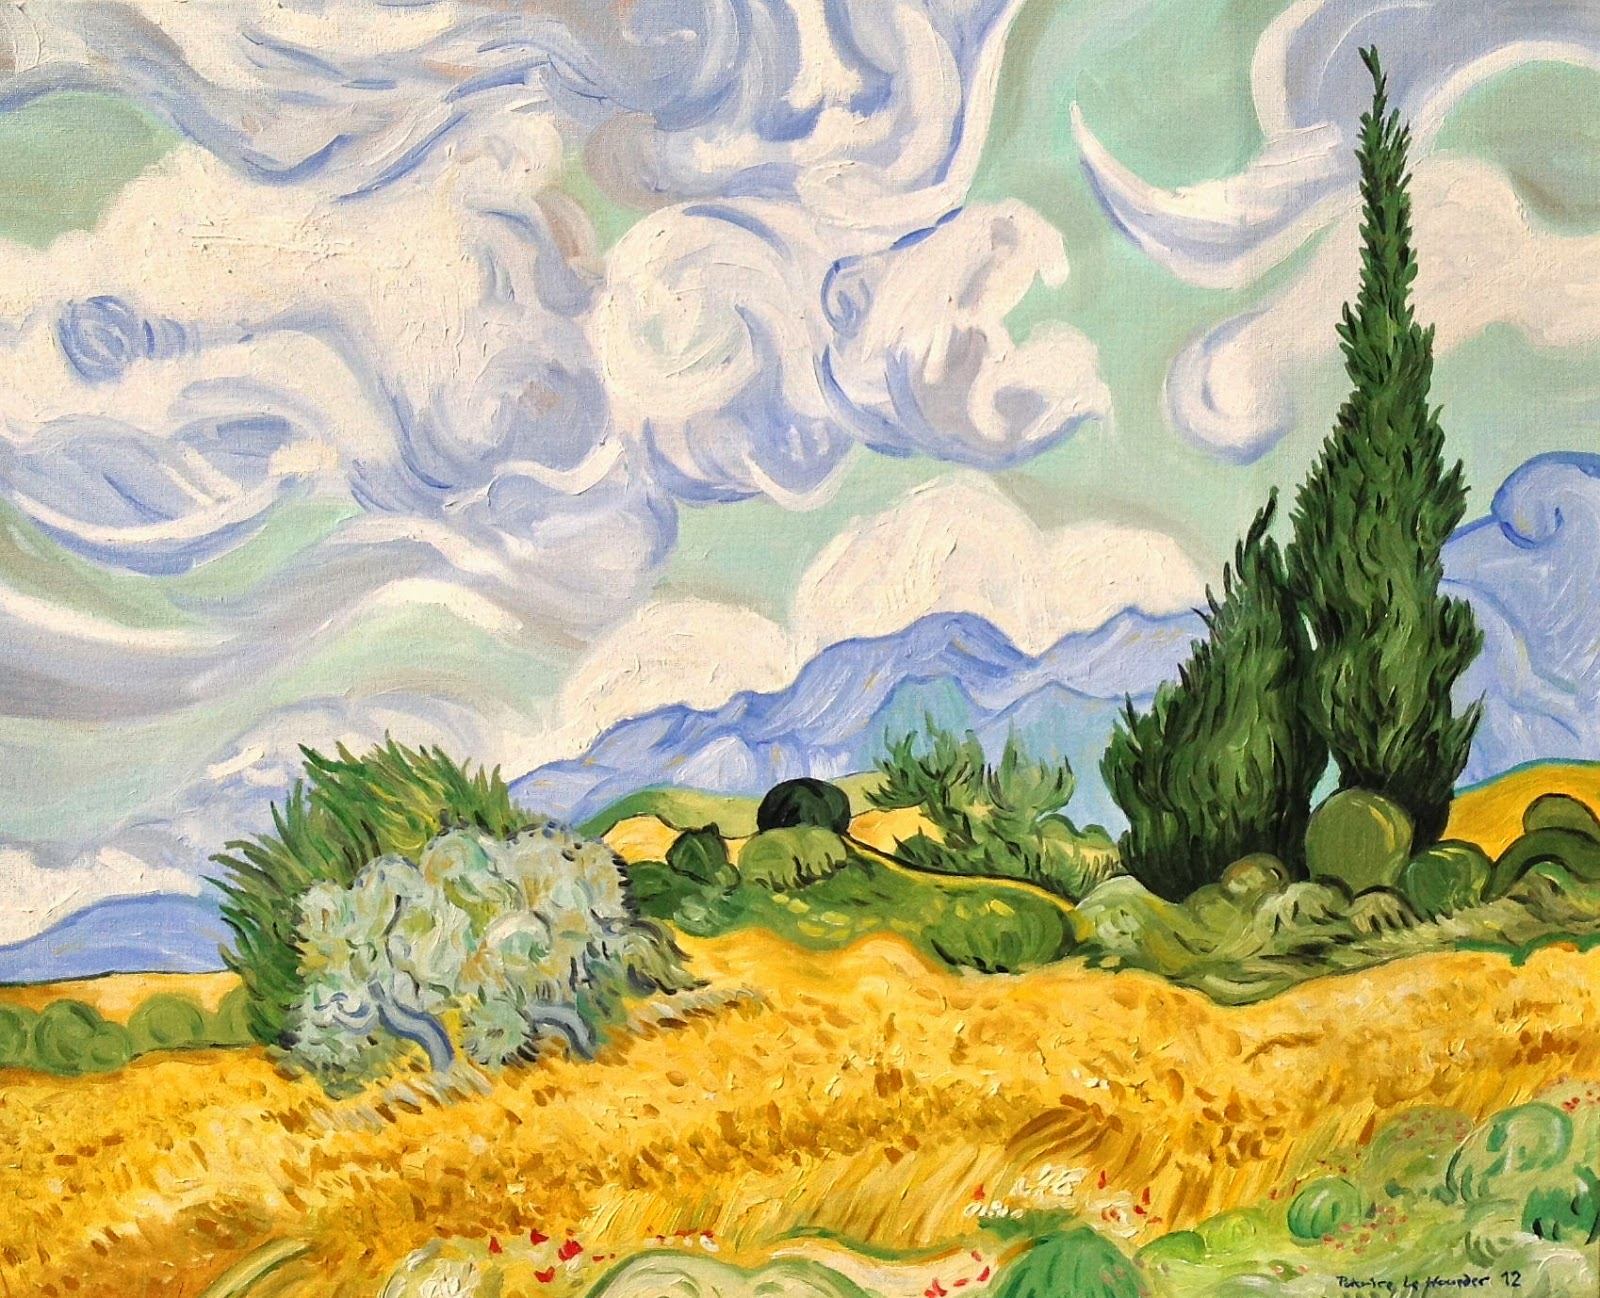
\includegraphics[scale=1.25]{v}}} % Image background
\centering
\vspace*{5cm}
\par\normalfont\fontsize{35}{35}\sffamily\selectfont
\textbf{Pokémon RPI\\Concept Design Document}\\
{\LARGE }\par % Book title
\vspace*{1cm}
{\Huge Aman Zargarpur\\Austin Gulati\\David Wang\\Tommy Fang}\par % Author name
\endgroup

%----------------------------------------------------------------------------------------
%	COPYRIGHT PAGE
%----------------------------------------------------------------------------------------

\newpage
~\vfill
\thispagestyle{empty}


\noindent \textsc{Pokémon RPI 2015, RCOS}\\

\noindent \textit{Published May 1st 2015} % Printing/edition date

%----------------------------------------------------------------------------------------
%	TABLE OF CONTENTS
%----------------------------------------------------------------------------------------

\chapterimage{pano-5.jpg} % heading image

\pagestyle{empty} % No headers

\renewcommand\contentsname{Pokédex}
\renewcommand{\bibname}{Bibliographie}
\tableofcontents% Print the table of contents itself

%\cleardoublepage % Forces the first chapter to start on an odd page so it's on the right

\pagestyle{fancy} % Print headers again

%----------------------------------------------------------------------------------------
%	CHAPTER 1
%----------------------------------------------------------------------------------------

\chapterimage{pano-5.jpg} % Chapter heading image

\chapter{Introduction}

\section{Introduction}\index{introduction}

  \vspace{1em}
The goal of this project is to create an open source game inspired by the older generations of Pokemon games,taking place on RPI campus.

  \vspace{2em}

\section{Road to BETA}

  \vspace{1em}
  	\begin{itemize}
		\item To Be able to explore multiple parts of campus.
  		\item Create interesting puzzles for player to solve.
  		\item Create meaningful story \& plot to maintain interest. 
        \item Creat tiles and patterns that match RPI.
  		\item Finish game, battle, animation engines
  		\item Finish Implementation of Terminal integration.
        \item Take photos and create color palette with RPI’s textures
        \ldots
	\end{itemize}
\newpage

%%%%%%%%%%%%%%%%%%%%%%%%%%%%%%%%%%%%%%%%%%%%%%%
\chapterimage{pano-5.jpg} % Chapter heading image

\chapter{Story Line}
%%%%%%%%%%%%%%%%%%%%%%%%%%%%%%%%%%%%%%%%%%%%%%%
\vspace{1em}
\indent The main storyline takes place in the same Pokémon world as the main series but in a different area. RPI is located somewhere far from the regions of Kanto (Blue/Red) and Sinnoh (Gold/Silver). These regions will be made first. Once we have the game engines polished, we can incorporate the game mechanics easily. Once we obtain beta status we can obtain feedback of the current game mechanics status and eliminate remaining bugs.

\vspace{1em}

\section{Main Game Spine - Archplot}
\vspace{1em}

\indent By implementing great plot and character development, the main character will obtain an “unconscious goal of desire” this goal will show how the main character triumphs over all the challenges at RPI and become a mature adult who has grown in his abilities. It will attempt to portray the lives we lead as students and how the work we do will pay off in the long run. This is my goal to tell the story like this.\\
\indent The game begins by welcoming the Class of 2018 and RPI theme song playing. Everyone who makes a new save file will begin as a freshmen regardless of actual class status. You will be able to pick your major, which will affect the exams you take (gym leaders that you fight throughout the game). The scene opens with Shirley telling you about the situation. The emergence of Pokémon in the real world has opened up entire realms of unanswered questions and things will never be the same again. Part of the Rensselaer plan has been revised in order to deal with these complex issues of “evolution” and supernatural powers that the Pokémon possess. It is your responsibility to utilize their abilities in order to create a better world. By training and capturing Pokémon for research, you become stronger and obtain more knowledge that will help you with your mission.\\
\indent Not all Pokémon will be used for good. Along the way, players will be approached by opposing trainers who are on the same quest to be the best that no one ever was. To catch them all is the real quest and to train them is the cause. You will travel across the land, searching far and wide. You must search the power that’s inside each Pokémon. It’s your destiny and Pokémon are your best friends in a world you must defend. Your courage will pull you through and the Pokémon will teach you and you will teach it. You will battle every day to claim your rightful place. Union College has joined the race and they want to destroy RPI students. Along the way, you will meet these students who will try to thwart your attempts to the best, but you will make their efforts futile.  
The new Pokémon training program is elite and rigorous. Players will have to obtain badges by passing each final in a semester. After you obtain 8 badges (2 badges for each class year), you must take a final graduation exam in order to test the strength of your resolve.


\section{Characters}

\vspace{1em}
In fictional literature, authors use many different types of characters to tell their stories. Different types of characters fulfill different roles in the narrative process.The following are our charcter types and the designs we intend to implement

\subsection{Protagonist:} The antagonist must be as strong as the protagonist. The wills of conflicting personalities must clash.\\
\subsection{Nemesis:} This is the “unified face of opposition” The entirety of the opposition experience by the protagonist. (Not just one antagonist, could be a collection or an experience)\\
\subsection{Pivotal character:} without a pivotal character, there is no play. This character moves the plot forward and this character knows what he wants. Without him, there is no story. Does not have to be the main character. (i.e. the joker, max payne)\\
\subsection{Mentor:} All the teachers, these characters will give you key advice on how to pass certain classes. I want to be able to offer good advice through the game. In your break time while you play this game, maybe you learn tricks to time management. These characters will also assist in backstory.
IF player talks to an NPC, dynamically bind NPC to appropriate chunk of script. Game remembers this state data in case there are future interactions.\\
\newpage
\subsection{procedurlly generated conversations}
“Player actions (killing a dragon, solving a mystery, and leveling up, buying new clothes) will seed the database with new conversational items—these then spread out like ripples in a pond. Developers can add new content both manually and programmatically, so rumors of a war might persist and grow for weeks before the armies actually get within sight. Like the childhood “whispering” game, where a phrase at one end of the room changes as it is whispered from child to child—exaggeration, substitution, and even mixing of rumors can take place on information stored this way. Players will feel a sense of integration into a larger whole, a real community—and intimately be part of your world as they see their own experiences woven into its history.”- (Sheldon (2013-04-03))
%%%%%%%%%%%%%%%%%%%%%%%%%%%%%%%%%%%%%%%%%%%%%%%%%%
\newpage


\chapterimage{pano-5.jpg} % Chapter heading image

\chapter{GamePlay Design}

%%%%%%%%%%%%%%%%%%%%%%%%%%%%%%%%%%%%%%%%%%%%%%%%%%%%

\vspace{1em}

\section {Level Design}
\subsection {Zone: ECAV/BARH}
	Your character will start in the ECAV gym where you will choose the starting Pokémon and pick up your room key. (Future implementation: residence hall choice) Possibly, you will be able to choose two starters from the 6 from Generations 1 and 2.  All of the starters begin at level 5. You will be given 10 Pokeballs and a Pokedex as well. Shirley will congratulate you on arriving here at RPI.  You are sent to your room where you have to talk to your RA and put away your things. The area between ECAV and BARH will be a low level Pokemon start zone inhabited by:\\
    \begin{itemize}
		\item Ratatat
  		\item Caterpie
  		\item Weedles
        \item Kakunas
  		\item Spinaraks
  		\item Pidgeys
        \item Hoothoot
        \item Digletts
        \item Ledybas
        \ldots
	\end{itemize}
 \indent There will be various items strewn across the map:\\
 \begin{itemize}
		\item Poke balls
  		\item potions
  		\item berries
        \item new trainers
        \ldots
	\end{itemize}
\indent After you arrive in your room, you can access your PC and store Pokémon. The PC will have many functions such as hall of fame checking (after you graduate), decorations for your room. There will be a Pokémon center and mart nearby.\\
\indent After becoming situated, you will receive a schedule (list of quests and tasks to do) from your RA. You’ve got a major test coming up, even though it’s your first day (WELCOME TO RPI.) You have to train in order to pass your first gym badge. [Add side quests and other characters for the player to do.] Campus tour function should be added also. You talk to a tour guide who gives you the map of RPI on the way out of your residence hall.\\
\indent The first quest is to visit the Union and find your student ID where you meet your rival. After this tutorial, you gain access to the rest of campus. This area is very huge and we should add specific characters that generate a lot of the back story. We go back to RPI’s founding in 1824. I’d like these characters to be talked to optionally. This allows exposition through choice which won’t force players to sit through the dialogue they don’t want to hear. Your first class begins in DCC 318. These are a series of Pokémon battles to test your strength and earn money. There is a maze here. Students will be blocking pathways and hiding items. This gives you a chance to explore and make the room less boring. The items set you up to the back hallways of the DCC building. (It’d be cool if we could implement the tunnels).

%%%%%%%%%%%%%%%%%%%%%%%%%%%%%%%%%%%%%%%%%%%%%%%%%%
\newpage


\chapterimage{pano-5.jpg} % Chapter heading image

\chapter{Core Mechanics}

%%%%%%%%%%%%%%%%%%%%%%%%%%%%%%%%%%%%%%%%%%%%%%%%%%%%


\section{Battle Mechanics}

\vspace{1em}
\subsection{Overview}
Players take turns battle each other using Pokémon. Each Pokémon has a specific learn set, which are moves that are learned after meeting a specific condition (leveling, evolution, etc…). In the original game, you could only have four moves at a time. Moves have limited uses called PP or power points. Power points decremented each time the move is used. They had to be restored using an item or by going to the Pokémon center. 
Each time you got a new move, you had to erase an old move. We plan on allowing players to keep all the moves in memory and having the ability to change learned moves when accessing a Pokémon center. Possible implementations include Move EXP and Move Levels. Players can carry up to six Pokémon on them. Catching Pokémon with a full team sends them to PC storage. The players can access PCs located in their home or Pokémon Center and other locations. Players can improve their growth through.
\subsection{Stats}
These stats are generated based on each Pokémon’s individual value(IV) and extra stats can be gained through attaining effort values(EV).\\

\includegraphics[scale=0.5]{stats.png}\\

\subsection{Hit points}
Pokémon’s life: when it reaches 0 in battle, the Pokémon faints and must be healed at the Pokémon Center. Certain items restore HP in or out of combat. Some moves deal damage based on HP.
\subsection{Attack}
Determines the power of physical attacks.(Bug, Fighting, Flying, Ghost, Ground, Normal, Poison, Rock or Steel-type)
\subsection{Speed}
Determines which Pokémon has first attack in battle. Some items, moves disregard this stat.
\subsection{Defense}
Resistance to physical attacks.
\subsection{Special Attack}
Increases the power of Special Attacks. (Dark, Dragon, Electric, Fire, Grass, Ice, Psychic, or Water-type)
\subsection{Formulas}
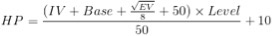
\includegraphics[scale=0.75]{f1.jpg}\\
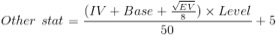
\includegraphics[scale=0.75]{f2.jpg}\\
\indent The stat is rounded down if the result is a decimal. Note that the numerator is multiplied by two compared to this formula before rounding. For example, the quantity (2*base + 2*IV + sqrt(EV)/4) is rounded down to the nearest integer before multiplying by level and dividing by 100. This is crucial to calculating the exact stats, as otherwise rounding errors will occur.
\subsection{Individual values}
IVs have a range from 0-15, in binary 0000-1111. HP IV takes the final binary digit of the Attack, Defense, Speed, and Special Ivs and places it that order.
\subsection{Effort Values}
Evs behave the same in Generation II as they did in Generation I. Both Special Attack and Special Defense share the EV for Special to maintain compatibility. The amount of Special Evs received is equal to the defeated Pokémon’s Special Attack base stat. 
Generation II introduced the Pokérus, a rare status condition which doubles the effort points gained in battle.
\subsection{Stat Modifiers}
Certain moves have special stat modifiers that decrease specific stats.\\
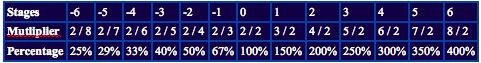
\includegraphics[scale=0.75]{mod.png}\\
This table shows the different stages of modifiers
\subsection{Critical Hit Chance}
Critical hits doubles move damage. Moves begin at stage zero.\\
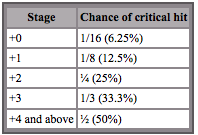
\includegraphics[scale=0.75]{crit.png}\\
\subsection{Weight}
 Weight affects the following game mechanics: 
 \begin{itemize}
 	\item Low Kick
 	\item Grass Knot
 	\item Heat Crash
 	\item Heavy Slam
 \end{itemize}
 Using a Heavy Ball modifies the catch rate of the targeted Pokémon depending on its weight.\\
Gold, Silver, and Crystal weight catch rates\\\\
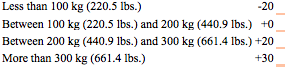
\includegraphics[scale=0.75]{weight.png}\\
\subsection{Status Effects}
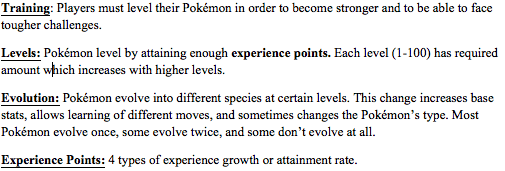
\includegraphics[scale=0.75]{se.png}\\
\section{Experience gain in battle}
\begin{itemize}
	\item The amount of experience gained in battle depends on the level and species of the defeated Pokémon in battle. The higher the defeated Pokémon’s level is, the more experience points it yields. The Exp. All and Exp. Share can also further affect the gain of experience.
	\item Gain more exp, if the player is in a Trainer battle.
	\item If winning Pokémon was traded from someone else
\end{itemize}
\subsection{slow}
\begin{itemize}
	\item The Slow group features the highest amount of experience required for a Pokémon to reach level 100 in Generations I and II, and the second highest amount since then. Containing many rare, powerful, and Legendary Pokémon, all pseudo-legendary Pokémon, by definition, are in this experience group. At level 100, a Pokémon in this experience group will have 1,250,000 experience points.
\end{itemize}
$$EXP = \frac{5n^3}{4}$$
\subsection{Medium Slow}
\begin{itemize}
	\item All normal starter Pokémon are in this group. Requiring 1,059,860 experience points for a Pokémon to reach level 100, it is the only experience group whose level 100 experience is not evenly divisible by 10,000.
\end{itemize}
$$EXP = \frac{6}{5}n^3-15n^2+100n-140$$
\subsection{Fast}
\begin{itemize}
	\item The Fast experience group is one of the four experience groups introduced in Generation I, with 800,000 experience points making for a level 100 Pokémon. Many Normal and Fairy-type Pokémon are in this group.
	\item For a list of all Pokémon in this group, see Pokémon in the Fast experience group
\end{itemize}
$$EXP = \frac{4n^3}{5}$$

\subsection{Medium Fast}
\begin{itemize}
	\item Requiring Pokémon to have an even 1,000,000 experience points to be at level 100, it is by far the most average of the experience groups, and the one with the simplest equation: to be at a given level, any Pokémon in this group requires experience equal to that level3. This group is also often called “cubic”, due to its function being a simple cube of the level.
	\item This experience group actually grows more slowly than the Medium Slow group up until about level 68 (level 47, if considering amount of experience required reaching the next level).
\end{itemize}
$$EXP = n^3$$
\newpage
\section{Type}
All moves/Pokémon have types which have strengths and weaknesses. During combat, Players should counter the opponent’s Pokémon type.\\
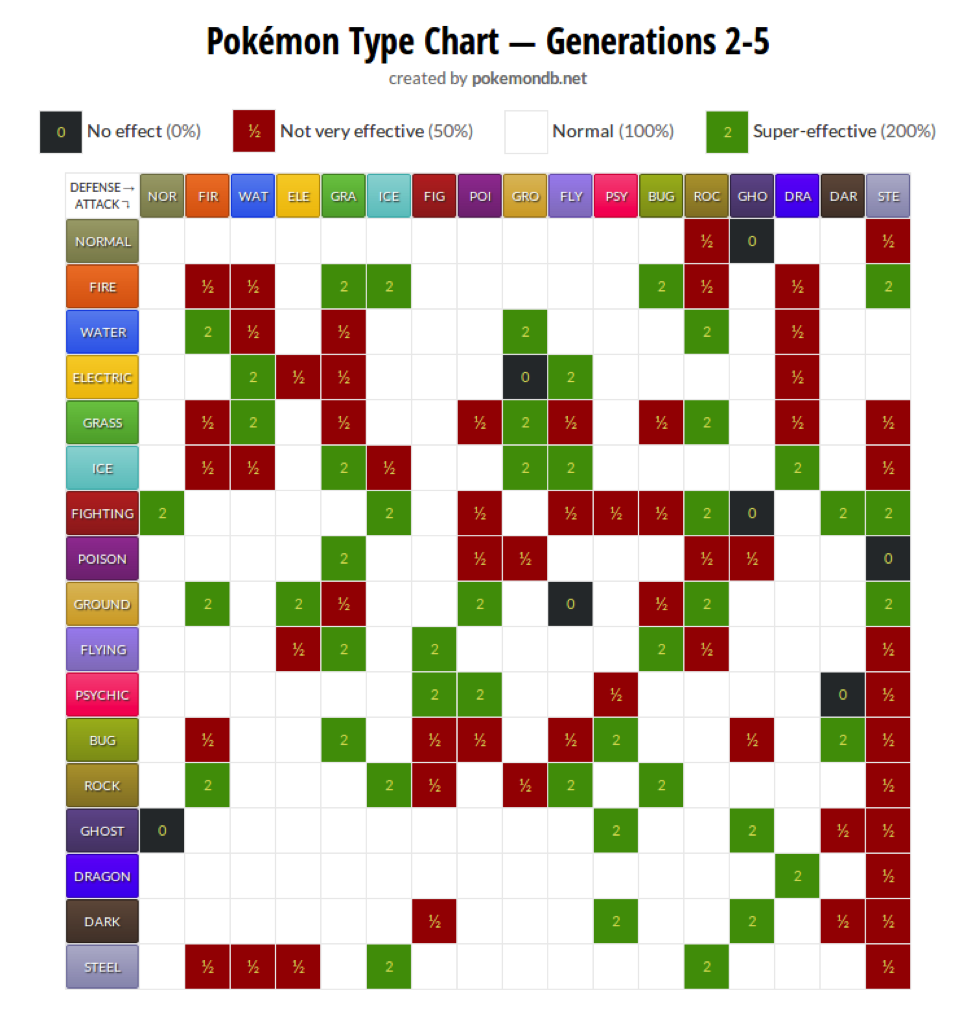
\includegraphics[scale=0.99]{sw.png}

% % % % % % % % % % % % % % % % % % %
\newpage

\chapterimage{pano-5.jpg} % Chapter heading image

\chapter{Plot Outline Draft}
% % % % % % % % % % % % % %
\section{Notes}
-Continuous Story Progression\\
-Team Rocket/Rival placeholder names.\\
1st Gym: \\
\indent DCC (Type counters water) \\
\indent – Leader: Prof. IHSS\\
2nd Gym:
Russel Sage (Type counters fire)
– Leader: Prof. Lynch
3rd Gym: 
Lally (Type counters grass) 
– Leader: Prof. Goldschmidt
4th Gym:
 Mueller Center (Type counters water)
– Leader: Prof. ATHLETIC DIRECTOR
5th Gym:
 Troy (Type counters grass)
– Leader: Prof. CIVIL
6th Gym:
 Pittsburgh Building (Type counters fire)
– Leader: Prof. PITTSBURGH
7th Gym:
 MRC Building (Type counters fire)
– Leader: Prof. MATERIALS
8th Gym:
 Amos Eaton (Type counters water)
– Leader: Prof. MATH
\section{Plots}
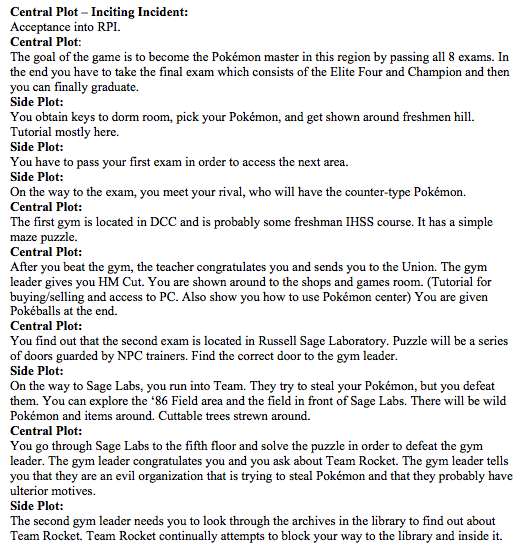
\includegraphics[scale=0.75]{p1.png}\\
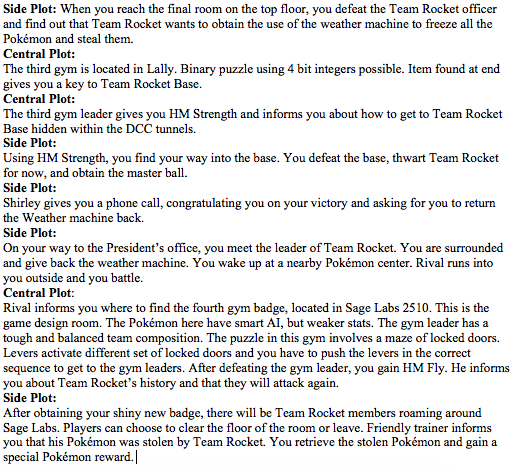
\includegraphics[scale=0.75]{p2.png}\\
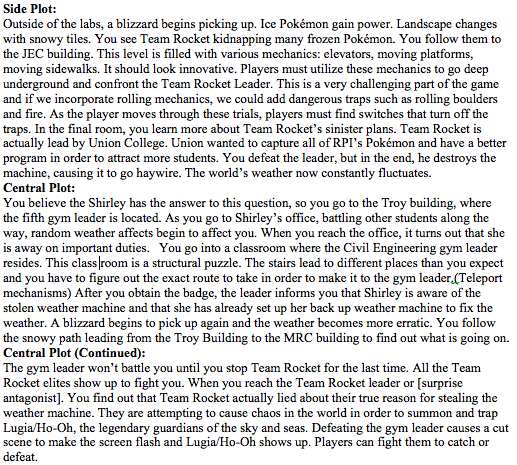
\includegraphics[scale=0.75]{p3.png}\\
Central Plot:
Elite Four ending goes here. Shirley congratulates you at The Approach for completing your 8 exams and lets you know that it’s not quite over yet. She lets the player know the location of the Elite Four in the EMPAC. You fight your way up The Approach and go to the EMPAC.
Elite One: Prof. ??
Elite Two: Prof ??
Elite Three: Prof??
Elite Four: Prof?? 
Elite Leader: Shirley?
Final Battle:
Shirley in the EMPAC.
Weather machine randomly changes, boosting powers of random type pokemon.
Team battle use powerful pokemon teamed with “WEATHERMACHINE”. This weather machine can cast all weather abilities.









\end{document}